\chapter{Combinations and interpretations of Run 1 searches for invisibly decaying Higgs bosons}
\label{chap:comb}
Whilst the \ac{VBF} production mode offers the best sensitivity to invisibly decaying Higgs bosons, the limits on \BRinv can be improved by taking into account searches performed using other production channels. Combinations with these other channels are described in sections \ref{sec:combotherchannels} to \ref{sec:combparked}. As well as combining the results of the \ac{VBF} searches with other channels, it is also possible to interpret them as limits on other specific models. Interpretations of the \ac{VBF} search results in several \ac{DM} models are described in \SectionRef{sec:dminterp}.

%??CHECK PLOT AXIS LABEL SIZES AND THAT LEGEND TERMS ARE STANDARD OR IN TEXT

\section{Searches in other channels}
\label{sec:combotherchannels}
%??Refer back to theory to introduce ZH and ggH searches
As described in \SectionRef{sec:higprod} after \ac{VBF} the next most sensitive production modes to invisible Higgs boson decays are \ac{ggH} and \ac{VH}. \ac{VH} has a much lower rate than \ac{VBF} (approximately 4 times less for a 125 \GeV Higgs boson). Compensating for this low cross-section, several of the final states of \ac{VH} production, particularly \ac{ZH}, give very clean signatures which are easy to identify. \ac{ggH} has a much higher rate than \ac{VBF}, but in most cases the resulting Higgs boson is created alone. However, if there is \ac{ISR} this can result in one or more jets allowing this channel to also be used. 

Three invisibly decaying Higgs boson searches were carried out by CMS during Run 1 in addition to the \ac{VBF} analyses. Two of these searches specifically targeted the \ac{ZH} production mode, one searching for events where the \PZ boson decayed to two leptons (the \PZ$(\ell\ell)$H search) and one where it decayed to two b quarks (the \PZ$(b\bar{b})$H search). The third ``monojet'' search targets events with one or more jets that are not \ac{VBF}-like and includes categories targeting \ac{ggH} and \ac{VH} production where the vector boson decays hadronically. 

%??signal fraction table
%??individual limits

When combining limits from separate analyses it is important that there is no overlap between the regions used by the analyses. A brief description of the event selection used in each of the non-\ac{VBF} invisibly decaying Higgs searches is therefore given in the following subsections. It is also important to understand which uncertainties are correlated between analyses and which are not. The uncertainties considered to be correlated between the analyses are discussed in Sections \ref{sec:combprompt} and \ref{sec:combparked}. 


\subsection{Z$(\ell\ell)$H$\rightarrow$invisible}
\label{sec:zllh}
%sel
The \PZ$(\ell\ell$)H search is described in Ref.~\cite{CMS-PAS-HIG-13-018}. The analysis selection requires two tight opposite charge same flavour leptons (either electrons or muons) both with \pt$>20$ \GeV, with invariant mass compatible with the \PZ boson, no further leptons and large \MET. Events containing two or more jets with \pt$>30$ \GeV are rejected to reduce the \PZ+jets background. 

To reduce backgrounds, in events with a single jet, that jet is required not to be identified using the \ac{CSV} algorithm (described in \SectionRef{sec:parkedtop}) as a b-jet. Also, requirements are made on the azimuthal angular separation and \pt balance between the \MET and the dilepton system. In addition to this signal region control regions, which differ from the signal region in that the lepton system is not compatible with a \PZ boson decay, are used for background estimation. Due to events with more than one jet being vetoed there is no overlap between the events in the signal or control regions of this analysis and the events selected in the \ac{VBF} and \PZ$(b\bar{b})$H analyses (where two jets with \pt$>30$ \GeV are required in all regions). 

%??limits

\subsection{Z$(b\bar{b})$H$\rightarrow$invisible}
\label{sec:zbbh}
%??sel
The \PZ$(b\bar{b})$H search is described in Ref.~\cite{CMS-PAS-HIG-13-028}. The analysis selection requires two jets tagged by the \ac{CSV} algorithm as originating from b-quarks, large \MET, and no reconstructed electrons or muons. The di-b-jet system is required to have high \pt, but low invariant mass (less than 250 \GeV). The dijet mass cut ensures there is no overlap with either of the \ac{VBF} analyses. The main background to the analysis is from \ac{QCD} multijet processes as in the \ac{VBF} analysis. Similarly to the selection of the parked data \ac{VBF} analysis this background is reduced using requirements on \jetmetdphi and \METsig. The neutral component of the \MET is also required to be aligned with the charged component in $\phi$. Control regions where the signal region selections are relaxed or inverted are used to estimate the remaining backgrounds.

%??limits

\subsection{Monojet searches}
\label{sec:monojet}
%??sel
The ``monojet'' search, is described in Ref.~\cite{CMS-PAS-EXO-12-055}. This analysis selects events with large \MET, one or more high-\pt jets and no reconstructed electrons or muons. To separate events due to \ac{ggH} production with \ac{ISR} from those due to \ac{VH} production where the vector boson decays hadronically, events are classified into three signal categories. The categorisation is sequential, i.e. if an event passes the requirements for the first category it is not considered for the second etc. 

The first category targets ``unresolved'' vector bosons where the high \pt of the vector boson causes its decay products to be very close together. These unresolved vector bosons are identified by searching for so-called ``fat'' jets with substructure with \pt$>200$ \GeV, (described in detail in Ref.~\cite{CMS-PAS-EXO-12-055}. One additional normal jet is allowed in this category as long as it is within 2 in $\phi$ of the fat jet.

The second category is the resolved category where the vector boson has lower \pt and its decay products can be identified as two separate normal jets. These jets are required to have an invariant mass between 60 and 110 \GeV, which overlaps with the range used in the \PZ$(b\bar{b})$H analysis regions, leading to a non-negligible overlap in the events selected. The resolved category is therefore not used in any combinations.

The third category is the ``monojet'' category. Events in this category are required to have one jet with \pt$>200$ \GeV. One additional jet within 2 in $\phi$ of the first jet is allowed to be present, with further jets causing the event to be vetoed. Control regions, which differ from the above categories by the presence of one or more leptons or photons, are used to perform background estimations. Finally, the category definitions above are not orthogonal to the \ac{VBF} analysis. To remedy this any events passing the \ac{VBF} parked data analysis selection were vetoed. As the monojet analysis was performed in 2015, after the parked data \ac{VBF} analysis had been performed, the monojet analysis was not combined with the prompt analysis. Therefore, no overlap veto between these two analyses was necessary.

The lepton veto present in all three signal categories means there is no overlap of any of the three categories with the \PZ$(\ell\ell)$H analysis regions. Some of the control regions do overlap slightly with regions of the \PZ$(\ell\ell)$H search, however these overlaps are very small due to the very high jet \pt cut present in the monojet search. In addition to the \PZ$(b\bar{b})$H search overlapping with the resolved category, there are also overlaps between the \PZ$(b\bar{b})$H search and the  unresolved and monojet categories. However, very few events in the \PZ$(b\bar{b})$H search have jets with \pt$>200$ \GeV, so these overlaps are considered negligible.

%??limits


\section{Combination with prompt VBF search}
\label{sec:combprompt}
%??Present combination
%??correlation decisions
%??interpolation

\begin{figure}
  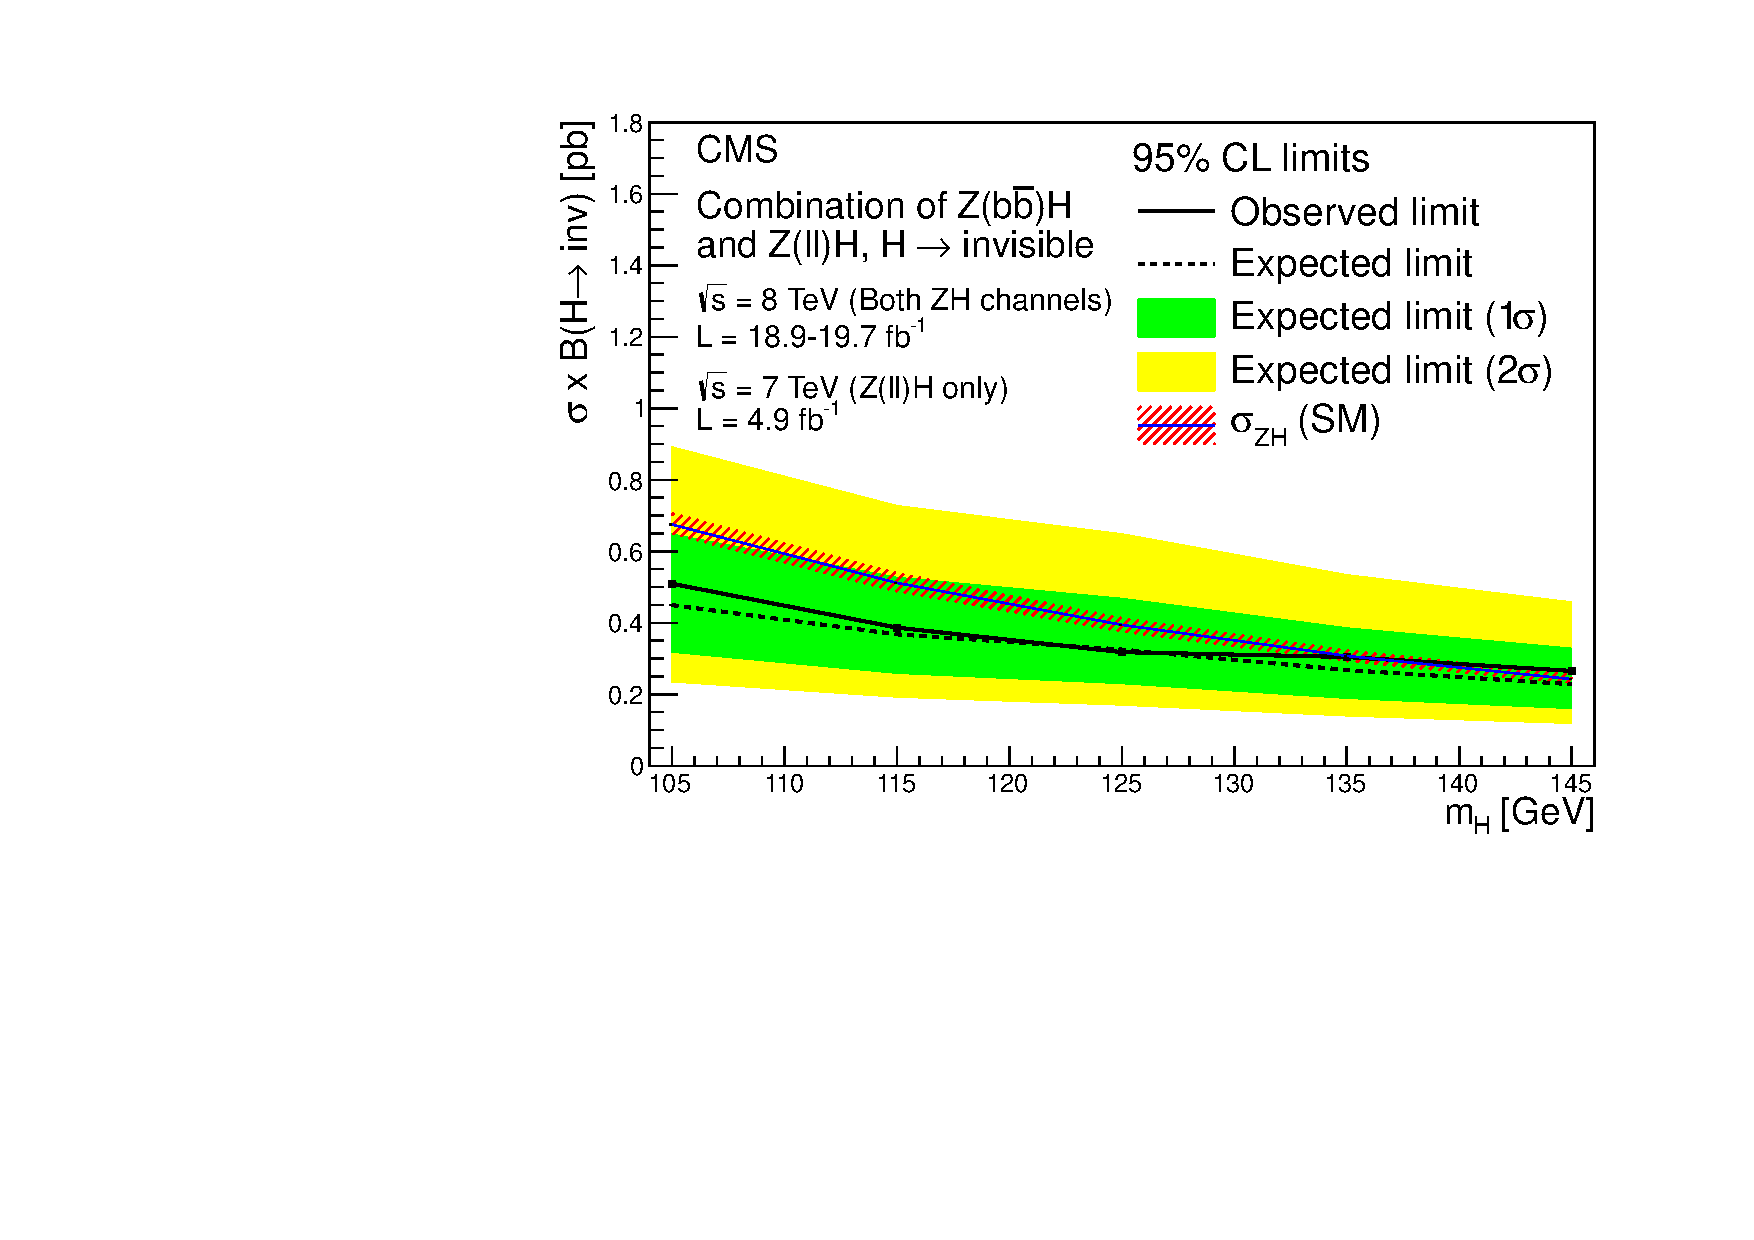
\includegraphics[width=.65\largefigwidth]{plots/prompt/HIG-13-30-figs/zhxslimit.pdf}
  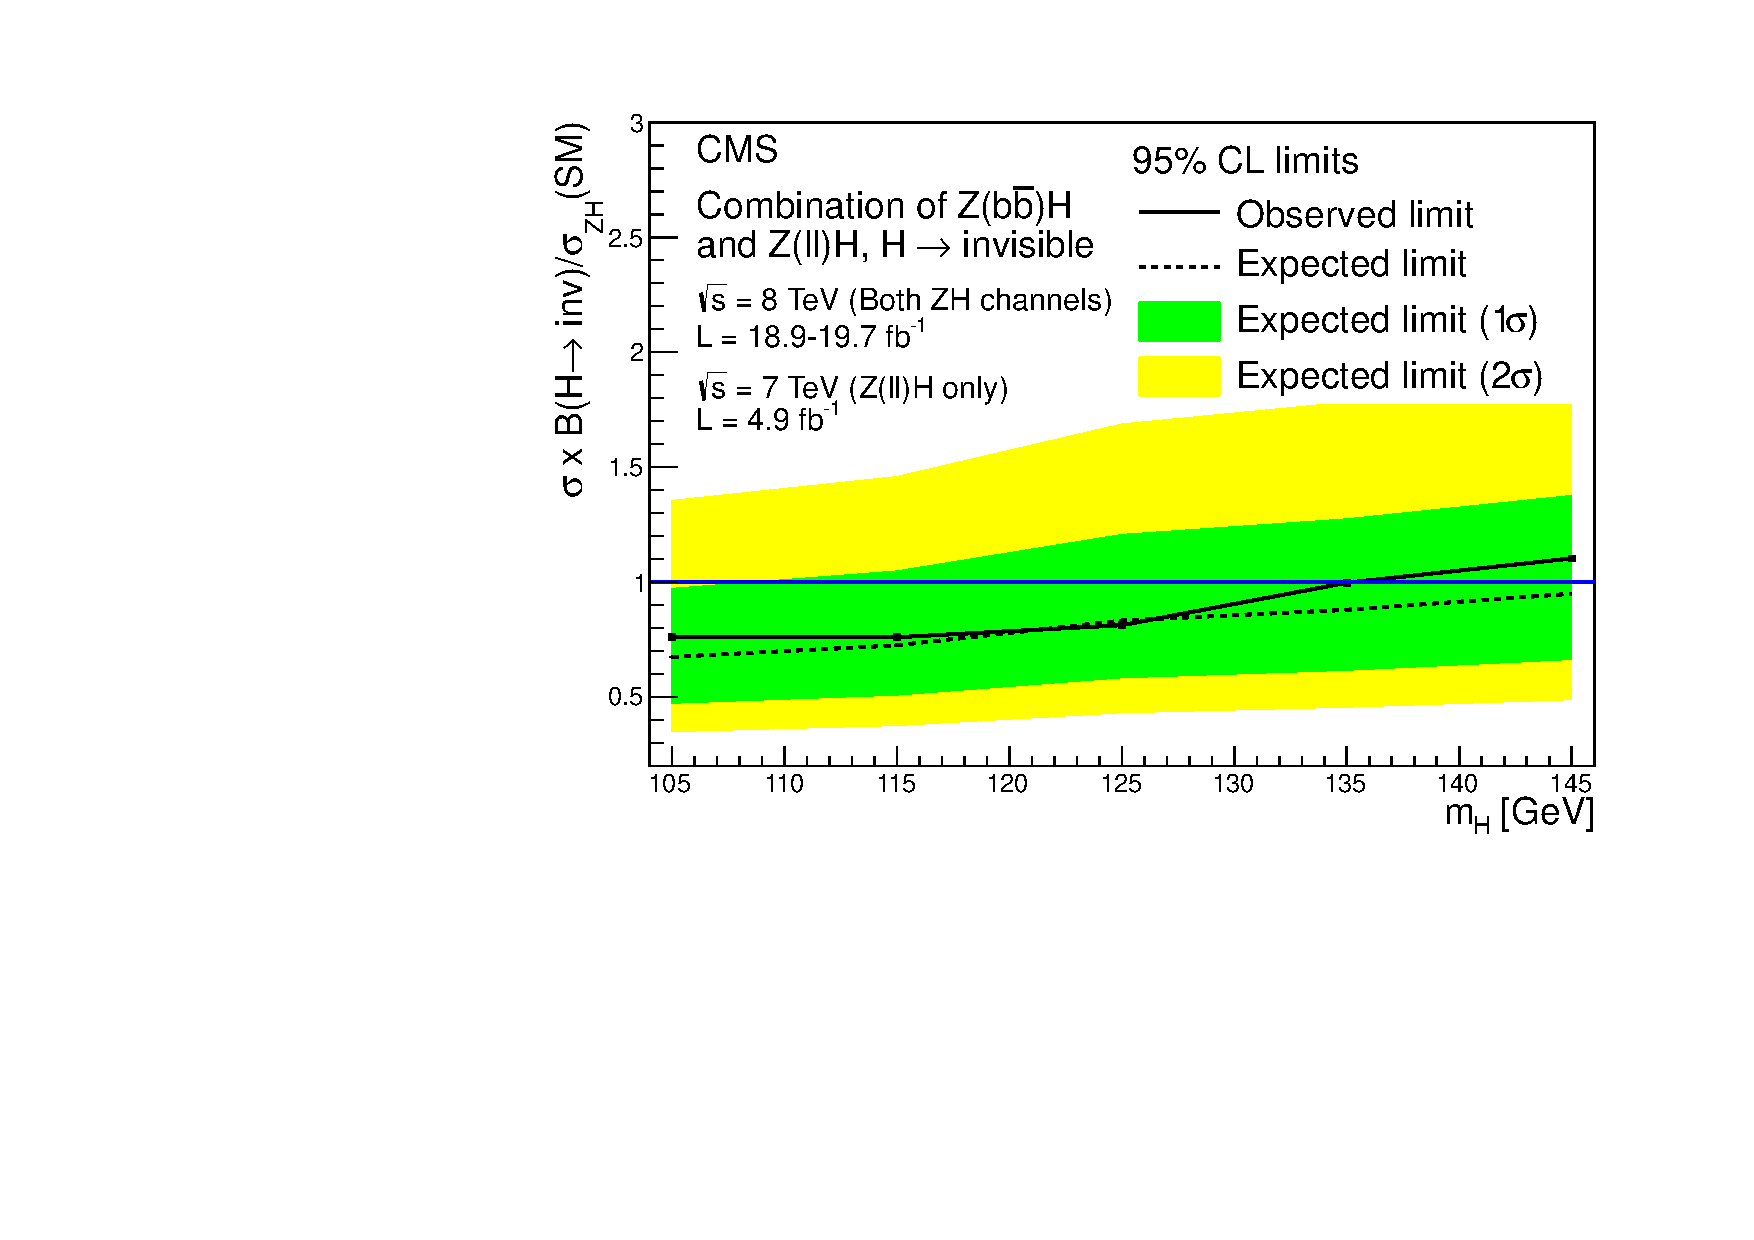
\includegraphics[width=.65\largefigwidth]{plots/prompt/HIG-13-30-figs/zhlimit.pdf}
  \caption{Expected and observed 95\% \ac{CL} upper limits on the \ac{ZH} $\sigma\times\mathcal{B}$ in \pb (a) and normalised to the SM \ac{VBF} Higgs boson production cross-section (b) obtained from the combination of the \PZ$(\ell\ell)$H and \PZ$(b\bar{b})$H searches~\cite{Chatrchyan:2014tja}. The green and yellow bands are the one and two sigma uncertainty bands of the expected limit.}
  \label{fig:zhcomb}
\end{figure}

\begin{figure}
  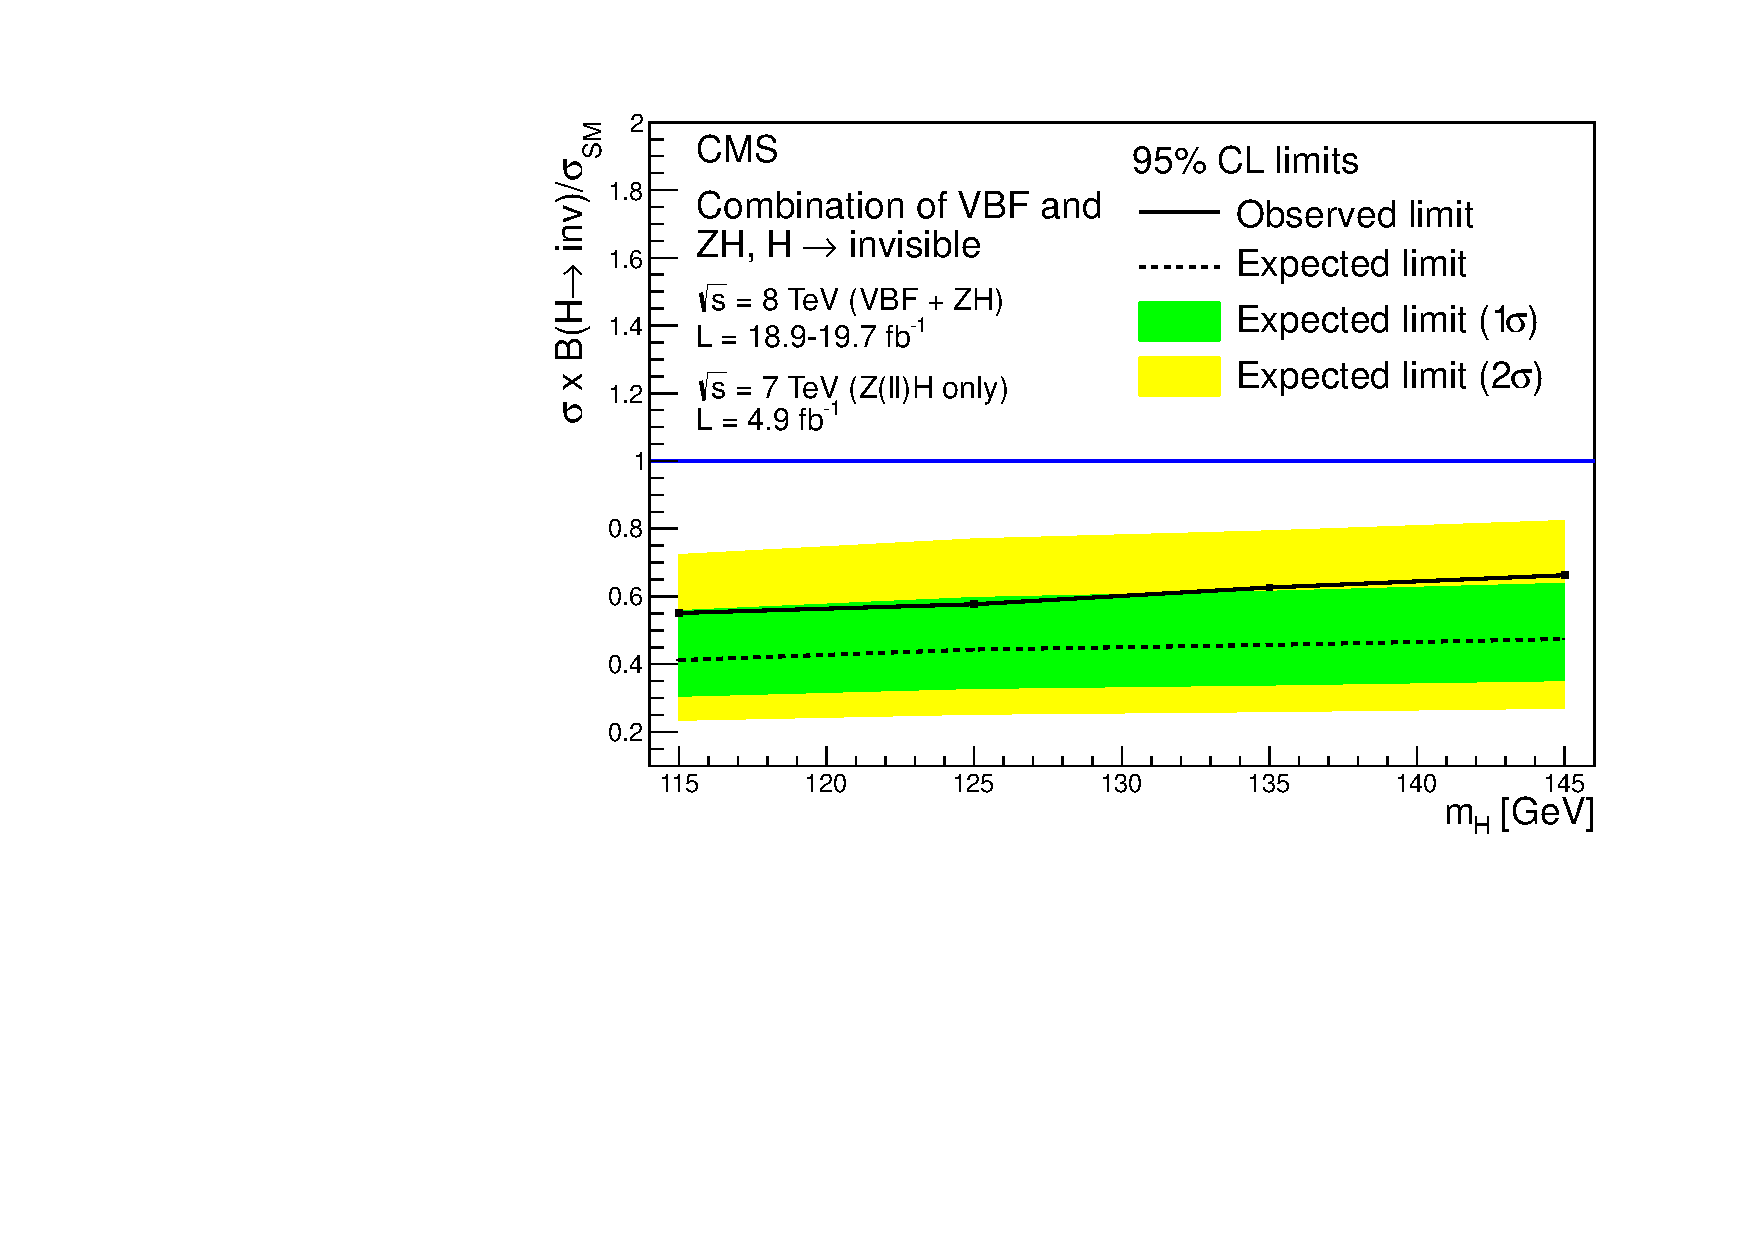
\includegraphics[width=\largefigwidth]{plots/prompt/HIG-13-30-figs/combinedlimit.pdf}
  \caption{}%??
  \label{fig:promptcomb}
\end{figure}

\begin{figure}
  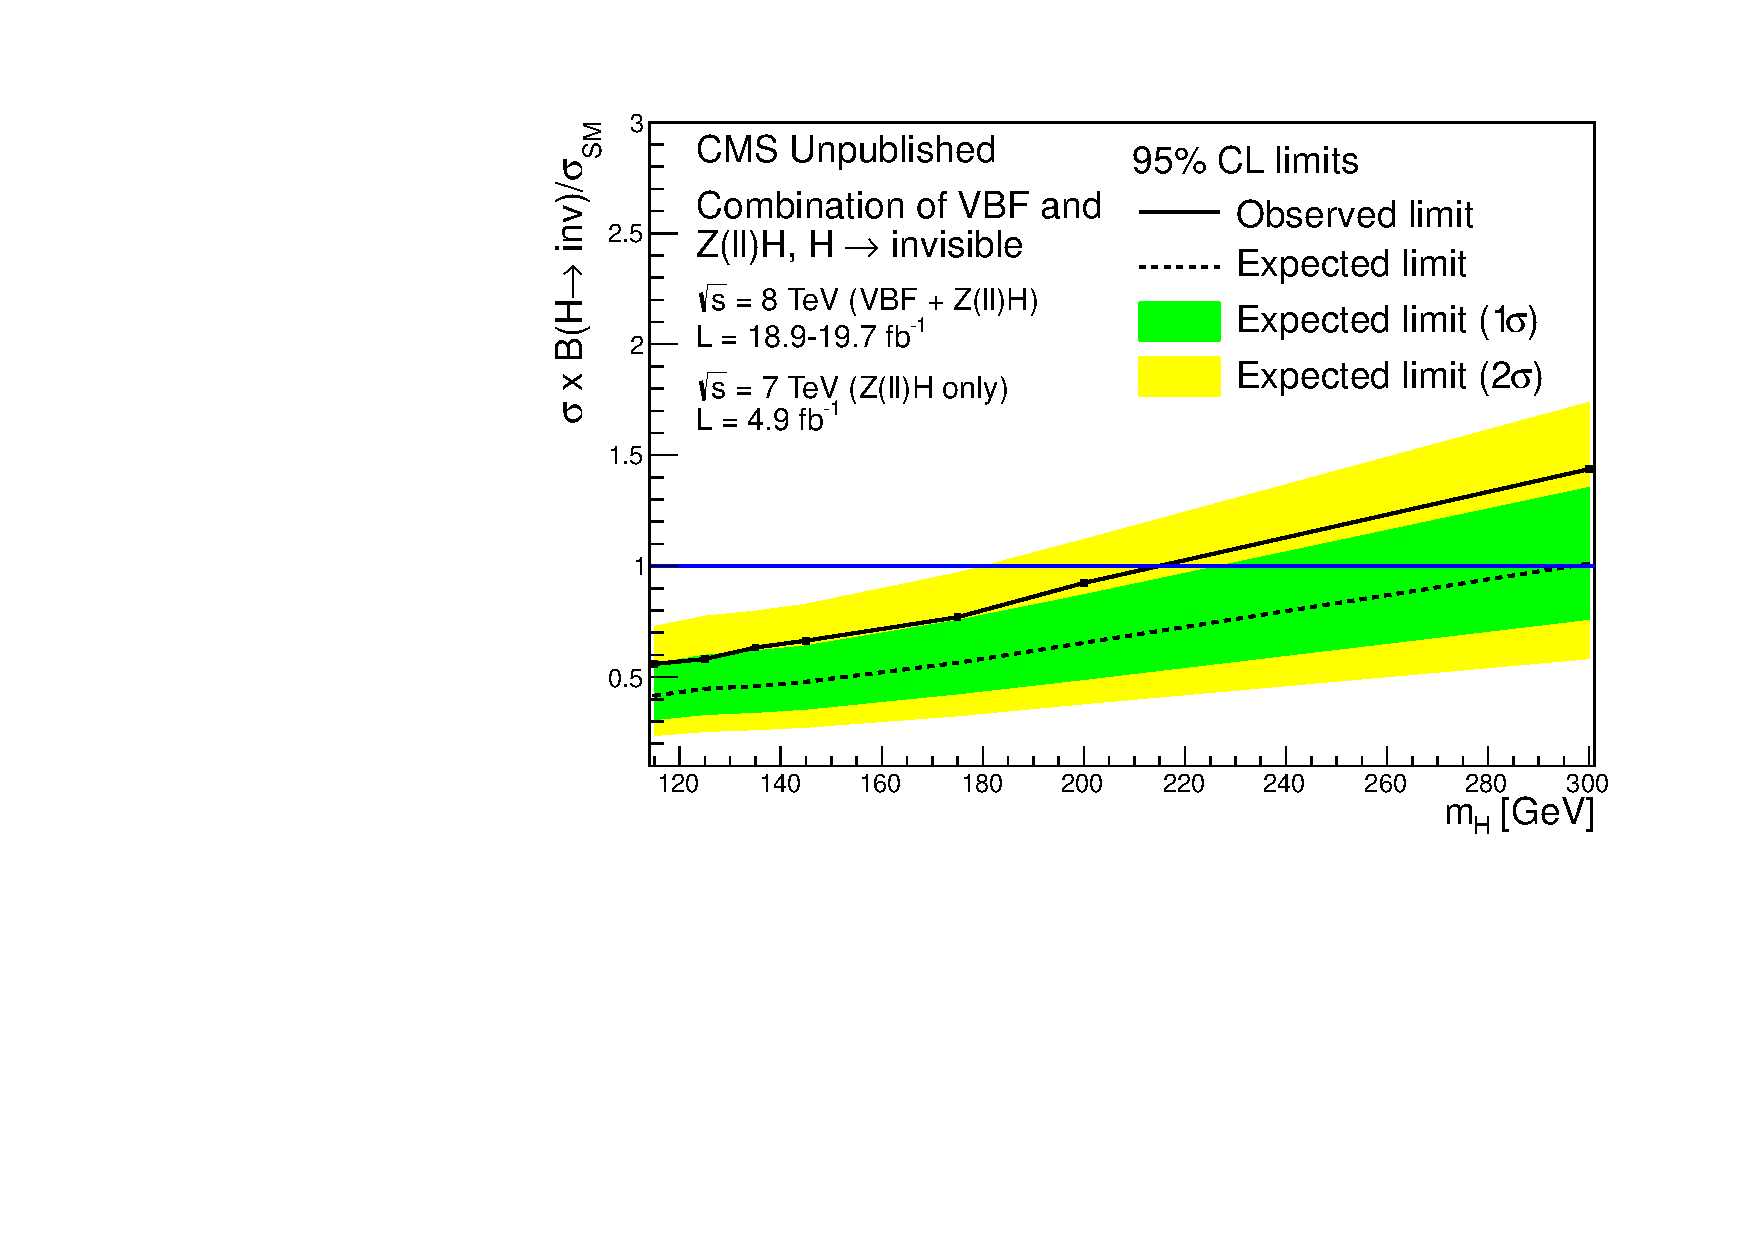
\includegraphics[width=\largefigwidth]{plots/prompt/HIG-13-30-figs/highmasslimit.pdf}
  \caption{}%??
  \label{fig:promptcombhighmass}
\end{figure}

\section{Combination with the parked VBF search}
\label{sec:combparked}
%??Present combination
%??syst studies, correlation of JES,JER etc. and why



\begin{figure}
  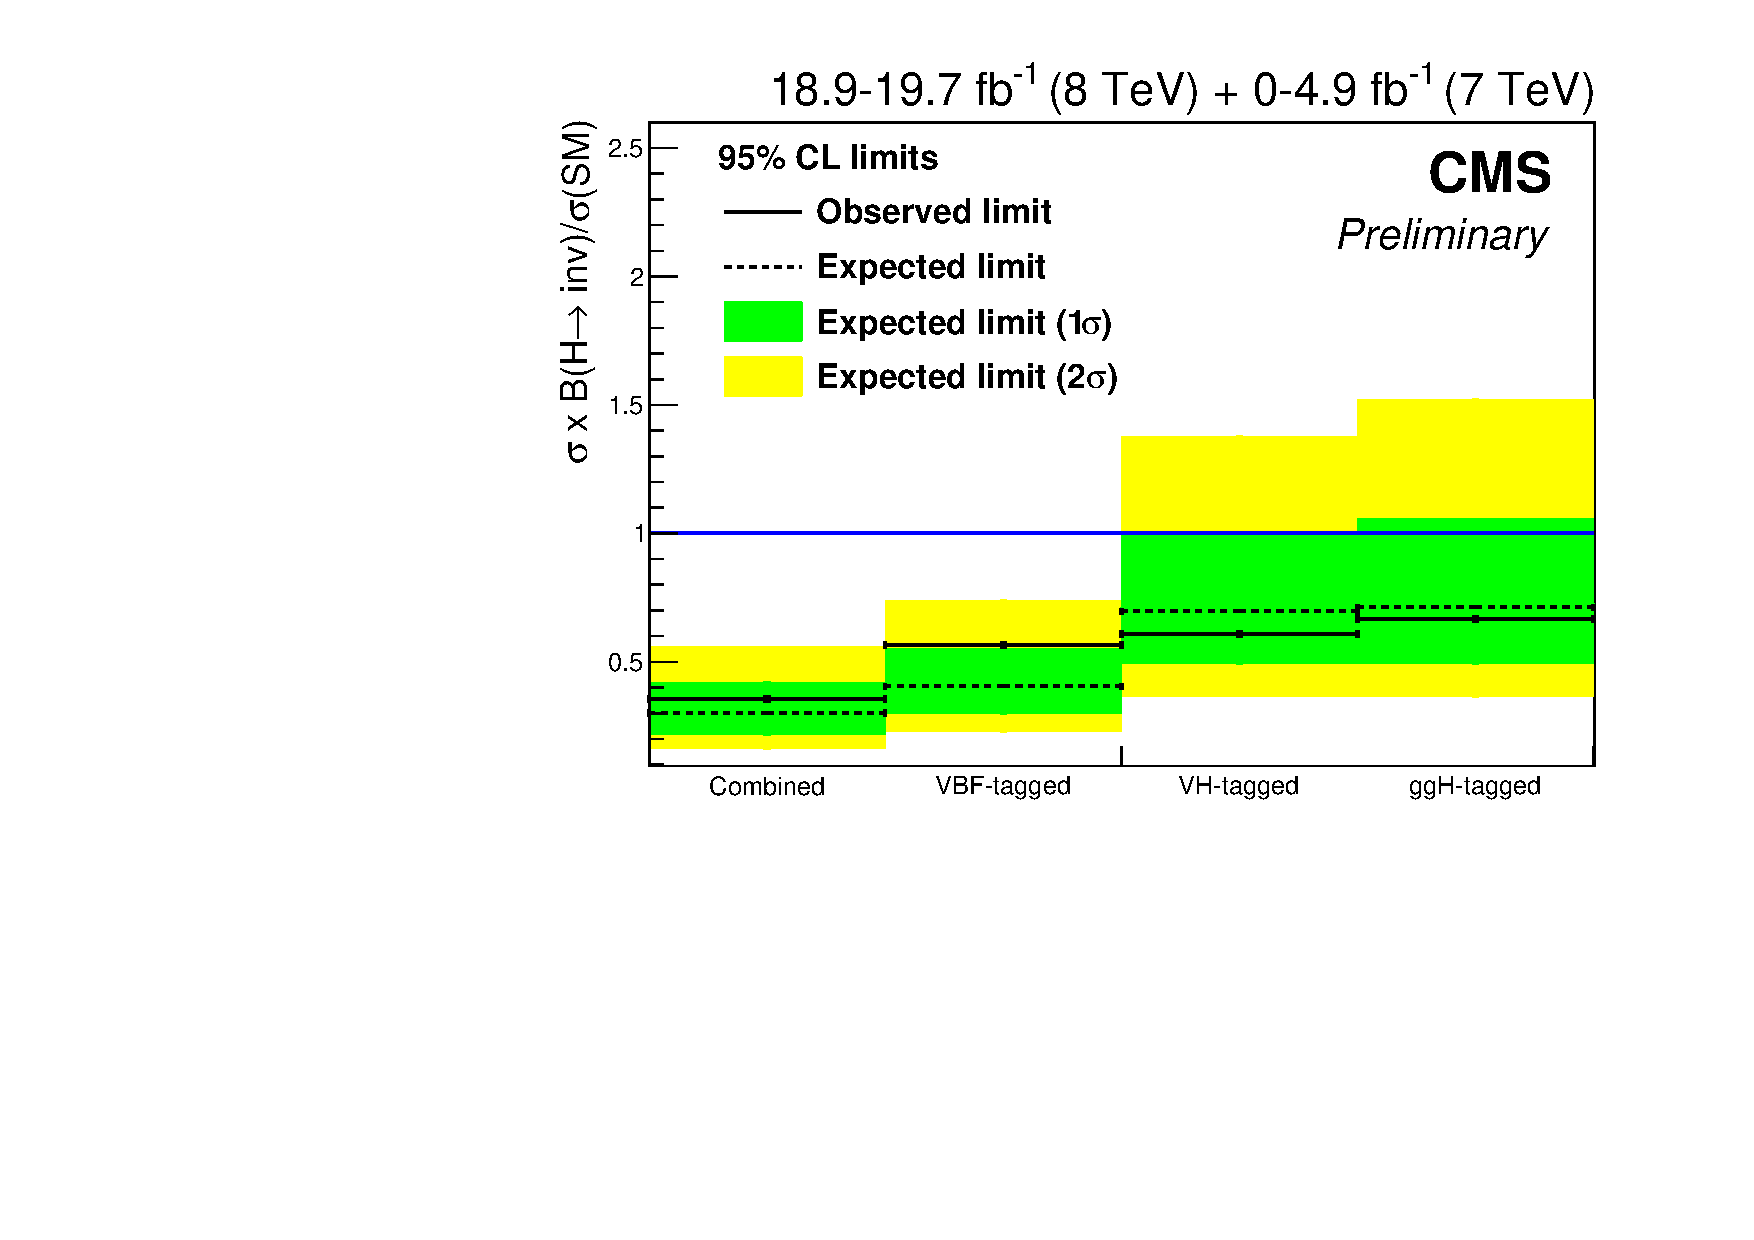
\includegraphics[width=\largefigwidth]{plots/comb/HIG-15-012-figs/channellimit.pdf}
  \caption{}%??
  \label{fig:parkedcombchannel}
\end{figure}

\begin{figure}
  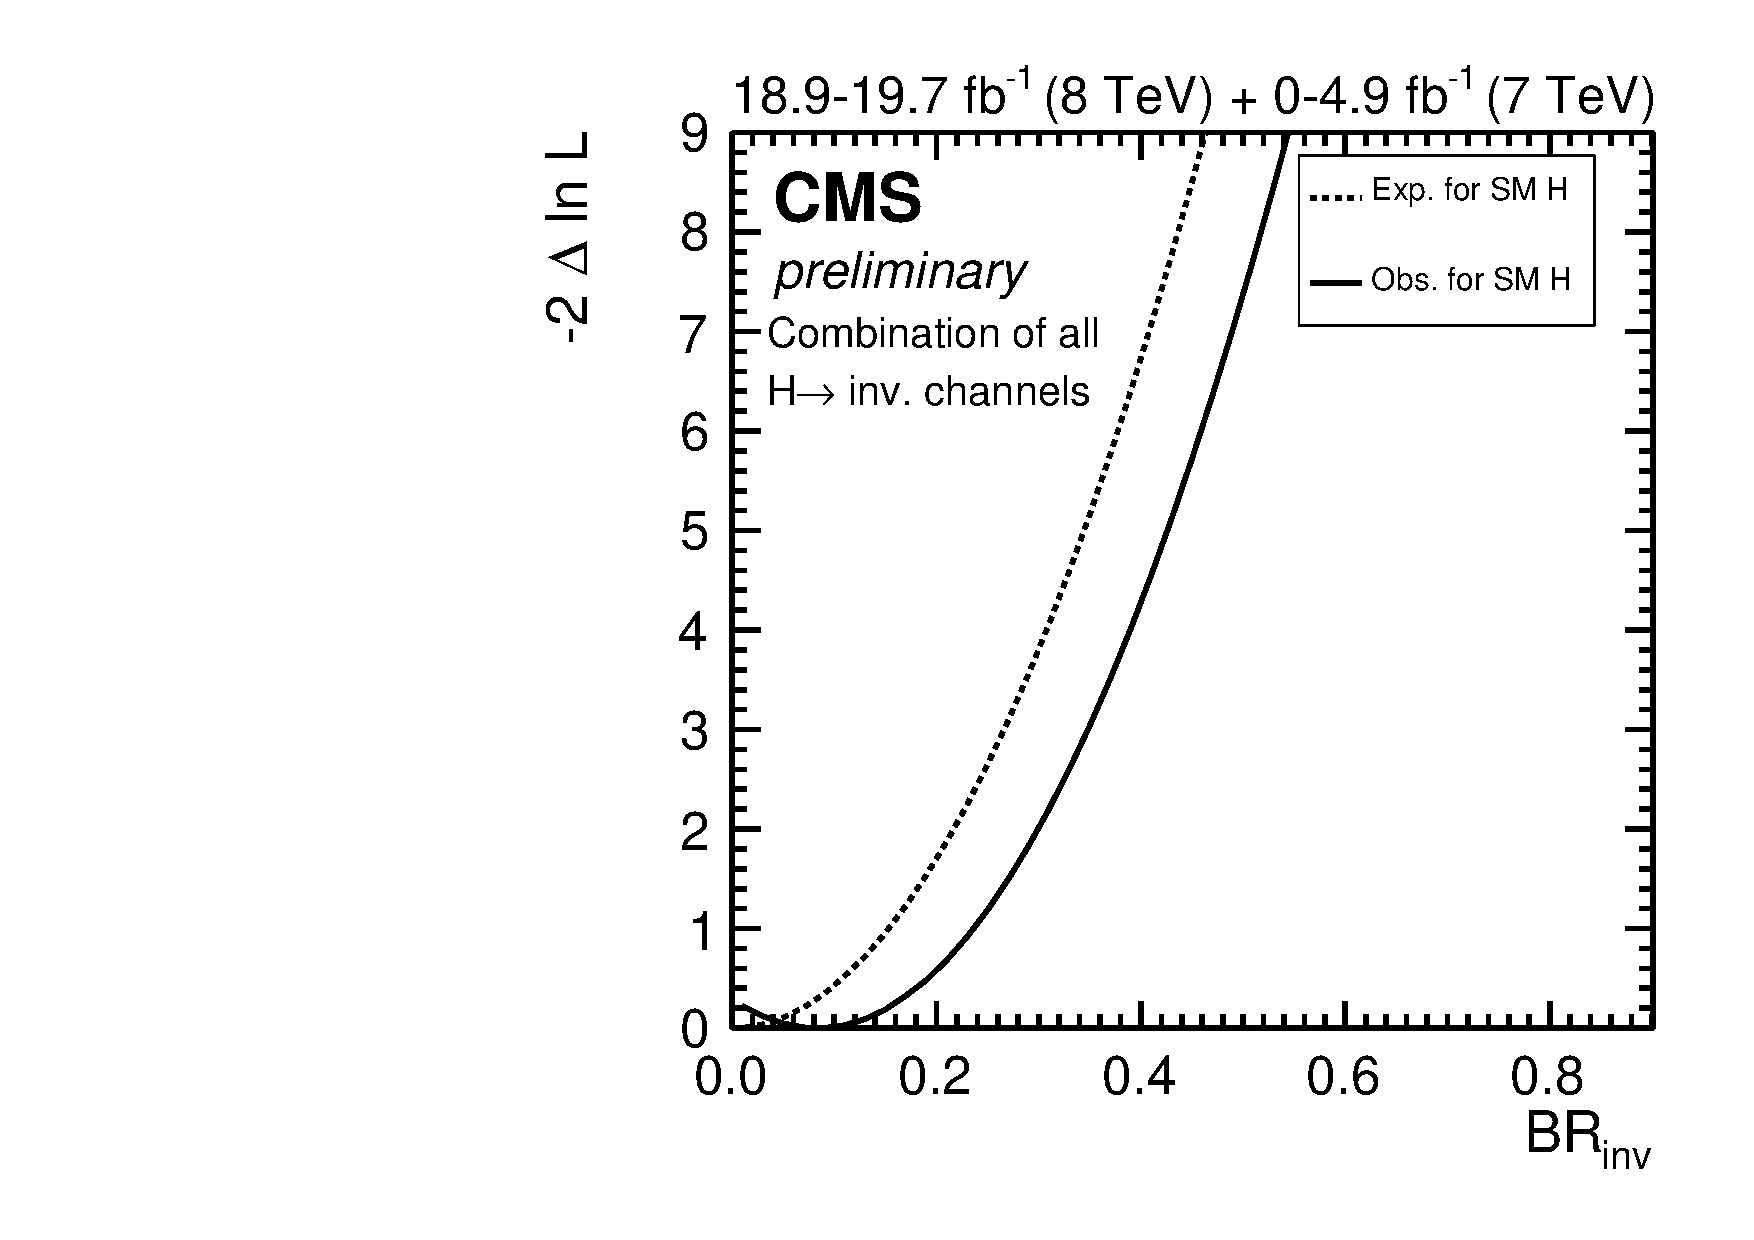
\includegraphics[width=\largefigwidth]{plots/comb/HIG-15-012-figs/combscan.pdf}
  \caption{}%??
  \label{fig:parkedcombscan}
\end{figure}



\section{Dark matter interpretations}
\label{sec:dminterp}
%??At minimum present an update of spin independent cross-section limit against dark matter mass plot from prompt data EPJC paper
%??Present progress on interpretations that is made between now and writing up
